\documentclass[a4paper]{article}

%% Language and font encodings
\usepackage[english]{babel}
\usepackage[utf8x]{inputenc}
\usepackage[T1]{fontenc}

%% Sets page size and margins
\usepackage[a4paper,top=3cm,bottom=2cm,left=3cm,right=3cm,marginparwidth=1.75cm]{geometry}

%% Useful packages
\usepackage{amsmath}
\usepackage{graphicx}
\usepackage[colorinlistoftodos]{todonotes}
\usepackage[colorlinks=true, allcolors=blue]{hyperref}

\title{Intro to AI: Heuristic Search}
\author{Brandon Smith \\ Nicholas Grieco}
\date{November 30th, 2017}

\begin{document}
\maketitle

\section*{Introduction}

This project delves deep into the different versions of the A* search algorithm. The algorithms are applied to grid-based maps that are difficult to traverse. When given a consistent heuristic function, A* is guaranteed to return the optimal path from goal to destination

\section*{a) Interface}
 
    By looking at the GUI, we can see that the heuristic value along the solution path is decreasing.

\section*{b) Abstract heuristic algorithm}

  \begin{figure}[!ht]
  \centering
  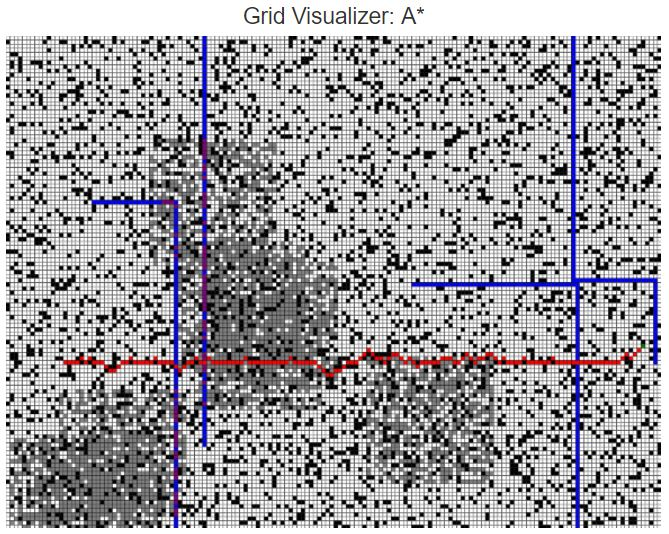
\includegraphics[width=150mm]{astar.JPG}
  \caption{\label{fig:Grid1}Example grid ran with A*}
  \end{figure}
  
  \begin{figure}[!ht]
  \centering
  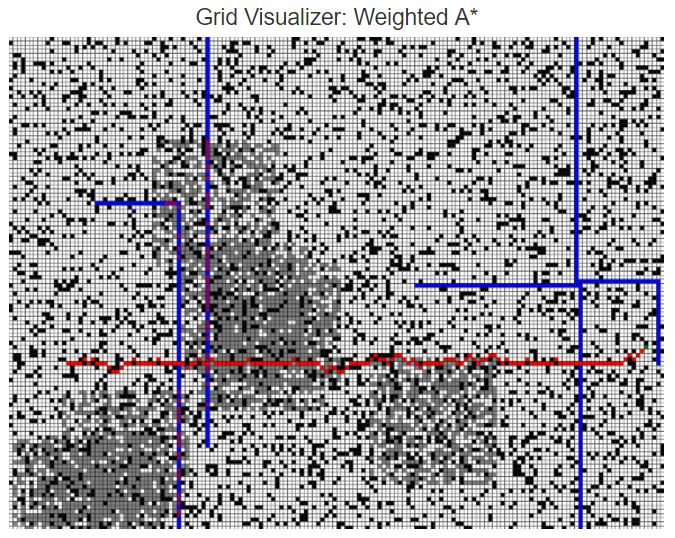
\includegraphics[width=150mm]{weighted_a_star_w_5.JPG}
  \caption{\label{fig:Grid2}Example grid ran with weighted A* (w = 5)}
  \end{figure}
  
  \begin{figure}[!ht]
  \centering
  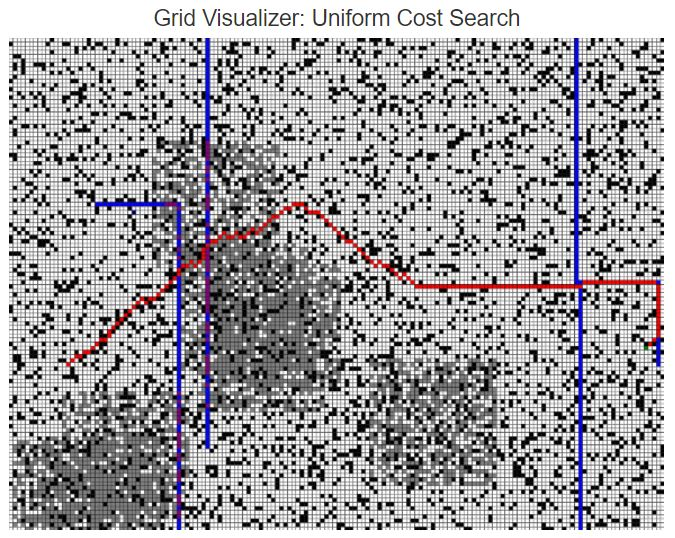
\includegraphics[width=150mm]{uniform_cost.JPG}
  \caption{\label{fig:Grid3}Example grid ran with uniform cost search}
  \end{figure}

\clearpage

\section*{c) Optimizations}
	\begin{itemize}
    \item Standard Euclidean distance is costly to compute due to the square root function. To decrease time to calculate Euclidean distance, an approximated square root value can be calculated.
    \item A closed list does not have to be maintained. This decreases search time and space of the closed list from O(n) to O(1). Each node has a visited flag which keeps track of its visited status. Rather than searching the visited list, you can directly see if a node has been visited.
    \item Using a binary tree as a priority queue decreases search and placing into the priority queue from O(n) to O(logn)
    \end{itemize}

\section*{d) Heuristic Variations}

Good heuristic functions can effectively guide the exploration process of a search algorithm towards finding a good solution fast and they are computationally inexpensive to compute. We propose 5 heuristic functions that will be useful for this problem.
\begin{itemize}
  \item Modified Euclidean. For our consistent and admissible algorithm we use a modified Euclidean distance algorithm. The fastest path that could ever be created between two points is a straight line along a river. This means that the best path would cost 1/4 * (euclidean distance). This scenario will not happen due to the constraints given on the formation of the rivers, however, it will never overestimate. By taking sample points along the 
  \item Example heuristic given. The example trace in section 4 of the assignment supplies a heuristic thats traced over a binary grid similar to our problem. 
  \item Manhattan Distance. The Manhattan distance is commonly used as a heuristic function. For our specific problem it is not admissible which implies not consistent as well. While its not guaranteed to underestimate every time, for this problem we hypothesize that it will still guide the search to the goal fast because it provides a relative distance to the goal compared to other cells that may be farther away.
  \item Averaging Manhattan and Euclidean. We assume that the Manhattan distance won't always give us an underestimate, however, we know that the modified Euclidean will never overestimate. By themselves, they each guide the search towards the goal, but by averaging them, we can reduce the number of times of overestimating. This can still lead to a possible increase in computation time.
  \item Chebyshev Distance. As a hybrid between Manhattan and Euclidean, Chebsyshev distances most directly fits our grid based mapping. Realistically, we can't always follow a straight line Euclidean distance because we are on a discretized mapping of cells. We can only make moves up/down, left/right and diagonal. The Euclidean distances goes through cells at different angles with moves that aren't necessarily legal moves. Chebyshev distance is used without a weighting factor which will cause it to not be admissible but should potentially increase decrease the search time of A*.
\end{itemize}

\section*{e) Benchmarks}

	See Tables 4-6
    
  \begin{figure}[!h]
  \centering
  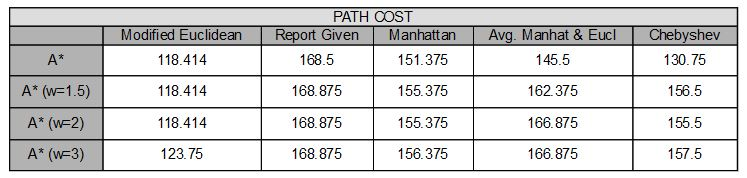
\includegraphics[width=150mm]{pathcost.JPG}
  \caption{\label{fig:Table1}Path cost of each algorithm with different heuristic functions}
  \end{figure}
  
  \begin{figure}[!ht]
  \centering
  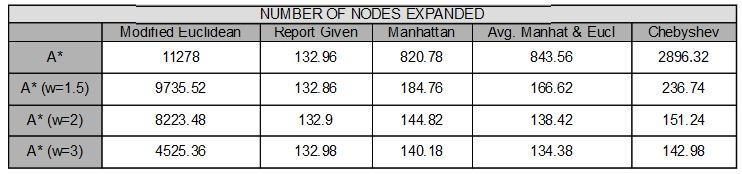
\includegraphics[width=150mm]{nodesexpanded.JPG}
  \caption{\label{fig:Table2}Number of nodes expanded by each algorithm with different heuristic functions}
  \end{figure}
  
  \begin{figure}[!h]
  \centering
  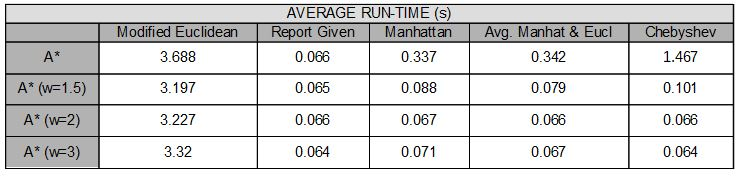
\includegraphics[width=150mm]{avgruntime.JPG}
  \caption{\label{Table3}Average run-time (in seconds) of each algorithm with different heuristic function}
  \end{figure}
  
  \begin{figure}[!h]
  \centering
  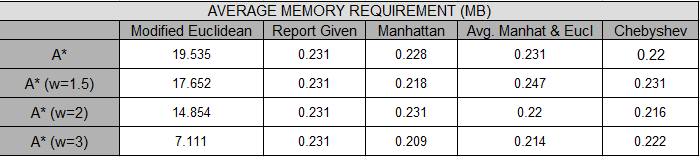
\includegraphics[width=150mm]{memory_req.png}
  \caption{\label{Table4}Average memory requirement (in MB) of each algorithm with different heuristic function}
  \end{figure}

\section*{f) Discussion}
It is clear that the modified Euclidean heuristic function provides the optimal solution every for every graph. The problem is that there is huge difference in time and memory required to calculate the optimal path compared with non-admissible heuristics.

By examining the tables, we can see that there is a direct correlation between the number of nodes expanded and the cost of the path. As the numbers of nodes expanded increases, the path cost decreases. This intuitively makes sense because as we see more paths we have the option of choosing better ones. Of course, this only correlation is only consistent until the optimal path is found and the cost cannot decrease any further. The average run-time and memory requirements generally follow the number of nodes expanded. This also makes sense because as we look at more nodes we will need more memory to keep track of the data and more time to process the information. The inadmissible heuristics give path lengths from 1.104-1.422 times the path cost of the optimal cost but return in only 1.78\%-39.7\% of the time. By using an inadmissible heuristic we get a slight longer path but the solution is calculated much faster. UCS takes roughly 3.65 seconds, expands 13634.18 nodes and return a path cost of 118.914. It takes just about the same time as generic A* and the same cost but it expands more nodes. Without a heuristic function we have no control over where the algorithm searches first. UCS is similar to A* with a heuristic cost of 0 for every node and it blindly searches all options. UCS's expands more nodes than all other algorithms and takes longer than all 4 other heuristic functions at a worse cost. UCS returns an optimal solution but is not the best approach for this type of problem.

Depending on the problem at hand, you have to decide between the trade-off between time and optimality. For this problem we believe that the best overall algorithm would be weighted A* with w=2 and using the Manhattan distance heuristic. It encompasses an overall good solution in terms of memory, path cost and runtime. The runtime is considerably faster than the consistent algorithm because the Manhattan heuristic value is calculated much quicker than the Euclidean distance due to its square root function. As for nodes expanded, its better than modified Euclidean and Chebyshev but slightly worse than the other 2. If your priority is optimality then choosing the consistent heuristic is the best choice. For speed, the best choice would be the one given in the report because it expands the least number of nodes but also returns the worst paths.

\section*{g) Sequential Heuristic A*}
	Sequential A* uses multiple inadmissible heuristics which causes it to have sub-optimality factor dependent on the w's given. We can see that the path costs below are larger than a majority of the algorithms in the previous section. It runs slightly faster than generic A* because it causes itself to stop early. Because it runs n + 1 searches its number of expanded nodes is less than the number of the other heuristics. If either the anchor terminates or an inadmissible search terminates, then the solution will be within a factor of w1*w2 of the optimal solution which is why the solution is not great and the search ends rather quickly.

\begin{figure}[!h]
  \centering
  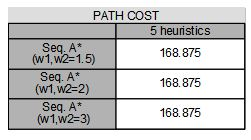
\includegraphics[width=60mm]{seqcost.JPG}
  \caption{\label{fig:Table1}Path cost of each algorithm with different heuristic functions}
  \end{figure}
  
  \begin{figure}[!ht]
  \centering
  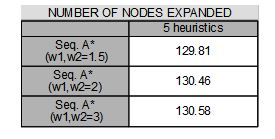
\includegraphics[width=60mm]{seqnodes.JPG}
  \caption{\label{fig:Table2}Number of nodes expanded by each algorithm with different heuristic functions}
  \end{figure}
  
  \begin{figure}[!h]
  \centering
  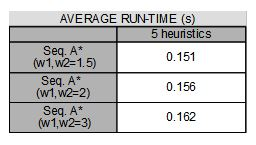
\includegraphics[width=60mm]{seqrun.JPG}
  \caption{\label{Table3}Average run-time (in seconds) of each algorithm with different heuristic function}
  \end{figure}



\section*{h) Efficiency}

It is extremely difficult to come up with a single heuristic function that encapsulates all of the complex information of a given search problem. Weights are being used on the heuristic function which makes it much more important because it has a greater influence on the search. Sequential A* uses different inadmissible heuristics in several searches that doesn't deteriorate the completeness of A* and also guarantees the bounds on the sub-optimality of the problem. The sub-optimality in determined by the two weight variables w1 and w2. w1 is used to put a weight on the heuristic for each of the searches and w2 determines to priority of the inadmissible searches over the anchor search.
\section*{i) Proof}

Considering the least cost path from start to goal as P. Pick a state that has not been expanded by anchor search but is in OPEN which will always be found. Thus we can follow the code below.

\begin{equation}
g_{0}(s_{i}) ≤ g_{0}(s_{i−1}) + c(s_{i−1}, s_{i}) 
\end{equation}
\begin{equation}
≤ w_{1} ∗ g^{∗}(s_{i−1}) + c(s_{i−1}, s_{i}) 
\end{equation}
\begin{equation}
≤ w_{1} ∗ (g^{∗} (s_{i−1}) + c(s_{i−1}, s_{i})
\end{equation}
\begin{equation}
= w_{1} ∗ g^{∗}(s_{i})
\end{equation}

Therefore, we derived 
\begin{equation}
g_{0}(s_{i}) ≤ w_{1} ∗ g^{∗}(s_{i})
\end{equation}

Continuing, we get

\begin{equation}
Key(s_{i}, 0) = g_{0}(s_{i}) + w_{1} ∗ h_{0}(s_{i})
\end{equation}
\begin{equation}
≤ w_{1} ∗ g^{∗}(s_{i}) + w_{1} ∗ h_{0}(s_{i})
\end{equation}
\begin{equation}
≤ w_{1} ∗ g^{∗}(s_{i}) + w_{1} ∗ c^{∗}(s_{i}, s_{goal})
\end{equation}
\begin{equation}
≤ w_{1} ∗ g^{∗}(s_{goal})
\end{equation}

If either the anchor terminates or an inadmissible search terminates, then the solution will be within a factor of w1*w2 of the optimal solution.

\begin{equation}
g_{0}(s_{goal}) ≤ w_{1} ∗ g^{∗}(s_{goal})
\end{equation}
\begin{equation}
≤ w_{1} ∗ w_{2} ∗ g^{∗}(s_{goal})
\end{equation}
\begin{equation}
w_{2} ≥ 1.0
\end{equation}

If the solution returns unsuccessfully then theres no finite cost solution.

\begin{equation}
g_{i}(s_{goal}) ≤ w2 ∗ OPEN0.Minkey()
\end{equation}
\begin{equation}
≤ w2 ∗ w1 ∗ g^{∗}(s_{goal})
\end{equation}










\end{document}